\section{Lecture 9. Pattern-Based Classification}

\subsection{Classification: Basic Concepts}

\begin{figure}[H]
    \centering
    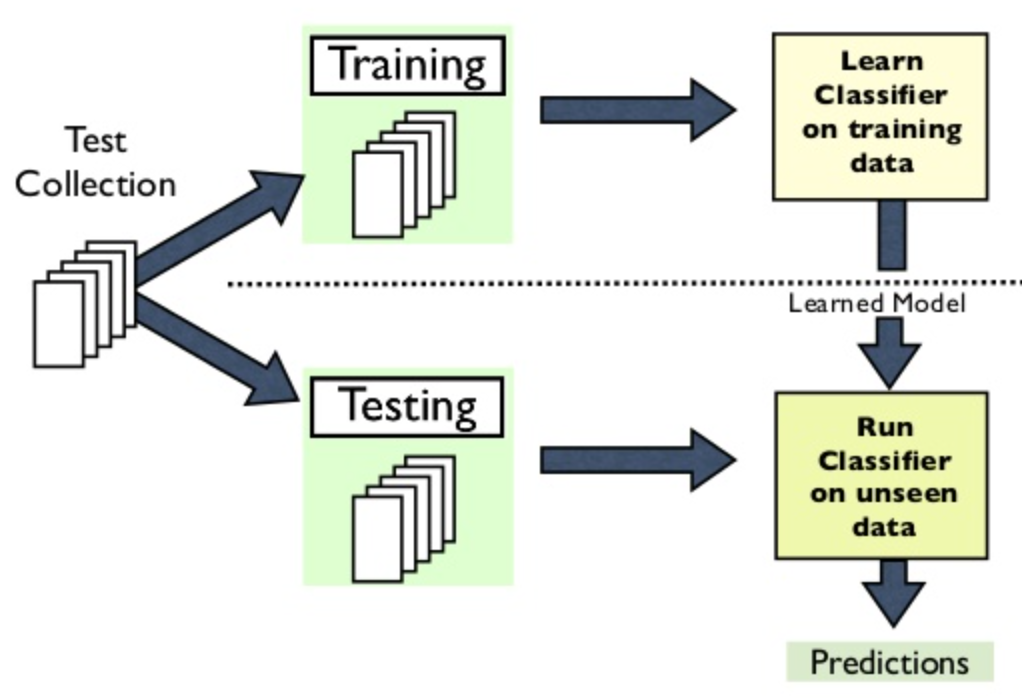
\includegraphics[width=0.7\linewidth]{classification.png}
    \caption{Classification}
\end{figure}

Typical Classification Methods:
\begin{itemize}
\item Support Vector Machines
\item Decision Tree
\item Neural Network
\item Bayesian Network
\end{itemize}

%--
\subsection{Pattern-based classification methods}
\begin{itemize}
\item CBA [Liu, Hsu \& Ma, KDD’98]: Use high-conf., high-support class association rules to build classifiers
\item Emerging patterns [Dong \& Li, KDD’99]: Patterns whose support changes significantly between the two classes
\item CMAR [Li, Han \& Pei, ICDM’01]: Multiple rules in prediction
\item CPAR [Yin \& Han, SDM’03]: Beam search on multiple prediction rules
\item RCBT [Cong et al., SIGMOD’05]: Build classifier based on mining top-k covering rule groups with row enumeration (for high-dimensional data)
\item Lazy classifier [Veloso, Meira \& Zaki, ICDM’06]: For a test t, project training data D on t, mine rules from $D_t$ , predict on the best rule
\item Discriminative pattern-based classification [Cheng et al., ICDE’07]
\end{itemize}

%--
\subsection{CBA: Classification Based on Associations}
\begin{itemize}
\item Mine high-confidence, high-support class association rules
\item LHS: conjunctions of attribute-value pairs); RHS: class labels\\
$p_1 \wedge p_2 ... \wedge p_l \to \left[A_{class-label} = C\right]$
\item Rank rules in descending order of confidence and support
\item Classification: Apply the first rule that matches a test case; otherwise apply the default rule
\end{itemize}

%--
\subsection{CMAR: Classification Based on Multiple Association Rules}
Rule pruning whenever a rule is inserted into the tree:
\begin{itemize}
\item Given two rules, $R_1$ and $R_2$, if the antecedent\footnote{Antecedent - предшественник} of $R_1$ is more general than that of $R_2$ and $conf(R_1) \geqslant conf(R_2)$, then prune $R_2$
\item Prunes rules for which the rule antecedent and class label are not positively correlated, based on the $\chi^2$ test of statistical significance
\end{itemize}

Classification based on generated/pruned rules:
\begin{itemize}
\item If only one rule satisfies tuple X, assign the class label of the rule \item If a ruleset S satisfies X
\begin{itemize}
\item Divide S into groups according to class labels
\item Use a weighted $\chi^2$ measure to find the strongest group of rules, based on the statistical correlation of rules within a group 
\item Assign X the class label of the strongest group
\end{itemize}
\end{itemize}

%--
\subsection{Discriminative Pattern-Based Classification}
\textbf{Principle:} Mining discriminative frequent patterns as high-quality
features and then apply any classifier.

Framework (\textbf{PatClass}):
\begin{itemize}
\item Feature construction by \textbf{frequent itemset mining}
\item Feature selection (e.g., using \textbf{Maximal Marginal Relevance (MMR)})
\begin{itemize}
\item Select \textbf{discriminative features} (i.e., that are relevant but minimally similar to the previously selected ones)
\item Remove redundant or closely correlated features 
\end{itemize}
\item Model learning: apply a general classifier, such as SVM or C4.5, to build a classification model
\end{itemize}

\subsubsection{On the Power of Discriminative Patterns}
K-itemsets are often more informative than single features (1-itemsets) in classification. Computation on real datasets shows: the discriminative power of k-itemsets (for $k > 1$ but often $\leqslant 10$) is higher than that of single features.\\

Computation on real datasets shows: pattern frequency (but not too frequent) is strongly tied with the discriminative power (information gain). Information gain upper bound monotonically increases with pattern frequency.

\begin{figure}[H]
\centering
\subfigure[IG vs. Pattern Length]{%
  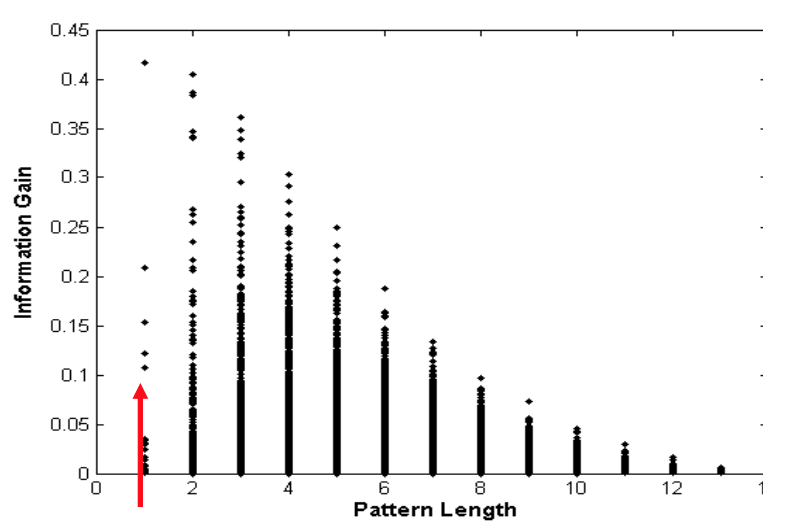
\includegraphics[width=0.42\linewidth, height=0.2\linewidth]{ig_len.png}
  \label{fig:ig1}}
\quad
\subfigure[IG vs. Frequency]{%
  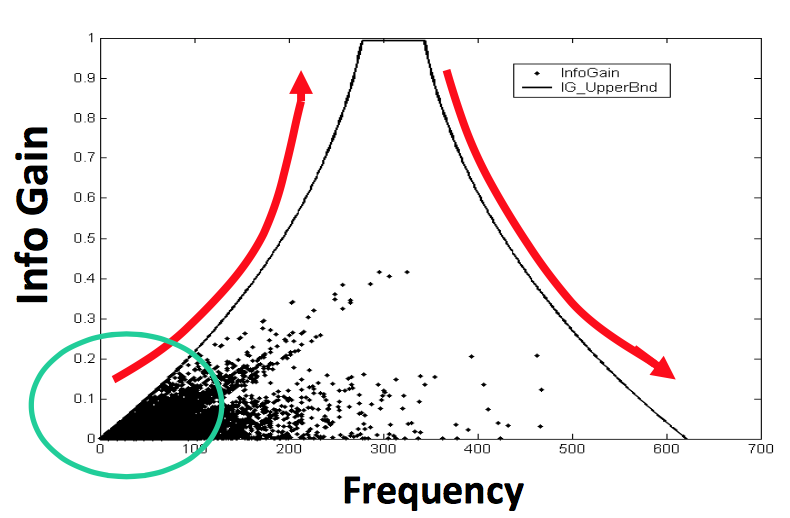
\includegraphics[width=0.42\linewidth, height=0.2\linewidth]{ig_freq.png}
  \label{fig:ig2}}
\caption{Information Gain}
\label{fig:ig}
\end{figure}

Information gain formula:
\begin{gather*}
IG (C \mid X) = H (C) - H (C \mid X)\text{, where }\\
H(C) = -\sum^{m}_{i=1}p_i \log_2(p_i)\text{ - entropy of given data}\\
H(C \mid X) = \sum_j P(X=x_j) H(Y \mid X=x_j)\text{ - conditional entropy of study focus}
\end{gather*}

%--
\subsection{DDPMine: Direct Mining of Discriminative Patterns}
General methodology:
\begin{itemize}
\item Input: A set of training instances D and a set of features F
\item Iteratively perform feature selection based on the \textbf{<<sequential coverage>>} paradigm
\begin{itemize}
\item Select the feature fi with the highest discriminative power
\item Remove instances Di from D covered by the selected feature fi
\end{itemize}
\end{itemize}

Implementation:
\begin{itemize}
\item Integration of \textbf{branch-and-bound search} with FP-growth mining
\item Iteratively eliminate training instances and \textbf{progressively shrink the FP-tree}
\end{itemize}

\subsubsection{Branch-and-Bound Search}
\begin{itemize}
\item The discriminative power (information gain) of a low frequency pattern is upper bounded by a small value
\item During FPGrowth mining we record the most discriminative itemset discovered so far and its information gain value $g_{best}$
\begin{itemize}
\item Before constructing a conditional FP-tree, we first estimate the upper bound of information gain based on the conditional DB
\item If the upper bound value $\leqslant g_{best}$, skip this conditional FP-tree and its subsequent trees
\end{itemize}
\end{itemize}



%--
\subsection{Recommended Readings}
\begin{itemize}
\item H. Cheng, X. Yan, J. Han \& C.-W. Hsu, Discriminative Frequent Pattern Analysis for Effective Classification, ICDE'07
\item H. Cheng, X. Yan, J. Han \& P. S. Yu, Direct Discriminative Pattern Mining for Effective Classification, ICDE’08
\item G. Cong, K. Tan, A. Tung \& X. Xu. Mining Top-k Covering Rule Groups for Gene Expression Data, SIGMOD’05
\item M. Deshpande, M. Kuramochi, N. Wale \& G. Karypis. Frequent Substructure-based Approaches for Classifying Chemical Compounds, TKDE’05
\item G. Dong \& J. Li. Efficient Mining of Emerging Patterns: Discovering Trends and Differences, KDD’99
\item W. Fan, K. Zhang, H. Cheng, J. Gao, X. Yan, J. Han, P. S. Yu \& O. Verscheure. Direct Mining of
Discriminative and Essential Graphical and Itemset Features via Model-based Search Tree, KDD’08
\item W. Li, J. Han \& J. Pei. CMAR: Accurate and Efficient Classification based on Multiple Class-association Rules, ICDM’01
\item B. Liu, W. Hsu \& Y. Ma. Integrating Classification and Association Rule Mining, KDD’98
\item J. Wang and G. Karypis. HARMONY: Efficiently Mining the Best Rules for Classification, SDM’05
\item X. Yin \& J. Han. CPAR: Classification Based on Predictive Association Rules, SDM’03
\end{itemize}

